% Festlegung des Allgemeinen Dokumentenformats
\documentclass[
a4paper, 			% Seitengröße
12pt,					% Schriftgröße
headsepline,	% Linie unter der Überschrift
ngerman,			% weiterleitung von deutscher Gramatik an andere Pakete
]{scrreprt} % mögliche Klassen: scrartcl, scrreprt, scrbook


% auslagern der imports in extra config datei
% Umlaut unter UTF-8 nutzen
\usepackage[utf8]{inputenc}

% Grafiken aus PNG Dateien
\usepackage{graphicx}

% Hilfspaket für Kopf- und Fusszeile
\usepackage{fancyhdr}

% Deutsche Rechtschreibung, Sonderzeichen und Silbentrennung
\usepackage[ngerman]{babel}

% Sonderzeichen Euro
\usepackage[right]{eurosym}

% Zeichenkodierung
\usepackage[T1]{fontenc}

% flüssigere Darstellung der Schriftart im PDF
\usepackage{lmodern}

% Textfarben
\usepackage{color}

% Mathematische Formeln und Ausdrücke
\usepackage{mathtools,amssymb}

% erstelle Inhaltsverzeichnis mit Querverweisen zu den Abschnitten
\usepackage[bookmarksnumbered, pdftitle={Dokumentation}, hyperfootnotes]{hyperref}
%\hypersetup{colorlinks, citecolor=red, linkcolor=blue, urlcolor=black}
%\hypersetup{colorlinks, citecolor=black, linkcolor= black, urlcolor=black}

% Zeilenabstand 
\usepackage{setspace}

% Zeilenabstand für Bildbezeichner
\usepackage{capt-of}

% Stichwortverzeichnis
\usepackage{makeidx}

% Stil der Zitierng
\usepackage[numbers,round]{natbib} % Runde Klammern

% Abkürzungsverzeichnis
% \usepackage[german]{nomencl}
\usepackage[printonlyused, withpage]{acronym} % Nur benuzte Akronyme ausgeben, mit Seitenzahl des ersten Auftrettens

% Paket für Tabellen
\usepackage{array}

% mehrseitige Tabellen
\usepackage{longtable}

% beliebig rotierbare Bilder ermöglichen
%\usepackage{floatflt}

% Packet für Seitenrandabstände
\usepackage{geometry}

% Paket für Boxen im Text
\usepackage{fancybox}

% fußzeile nummerierung nicht reseten
\usepackage{chngcntr}

% override numbering of sections
% \usepackage{titlesec}
% set depth to 4; 1. chapter -> 1.1 section -> 1.1.1 subsection -> 1.1.1.1 subsubsection -> 1.1.1.1.1 paragraph
% \setcounter{secnumdepth}{4}


% Kopf- und Fusszeile
% Kopf- und Fusszeile erzeugen
% erstelle eigenen Seitenstil
\pagestyle{fancy}

% bereinige Kopf- und Fusszeilenfelder
\fancyhf{}

% Kopfzeile
\fancyhead[L]{\nouppercase{\leftmark}} % Kopfzeile Links
\fancyhead[C]{} % Kopfzeile Mitte
%\fancyhead[R]{\thepage} % Kopfzeile Rechts
\renewcommand{\headrulewidth}{0.4pt} % Trennlinie oben

% Fußzeile
% \fancyfoot[L]{} % Fußzeile Links
% \fancyfoot[C]{\thepage} % Fußzeile Mitte
\fancyfoot[R]{\thepage} % Fußzeile Rechts
% \renewcommand{\footrulewidth}{0.4pt} % Trennlinie Unten

% diverse Dokument Einstellungen
% Einstellung für Seitenränder
\geometry{left=3cm, right=2.5cm, top=2.5cm, bottom=3cm}

% Indexerstellung
\makeindex

% Beginne Dokument
\begin{document}
	
	% Leere Seite am Anfang
	% \thispagestyle{empty} % erzeugt Seite ohne Kopf- / Fusszeile
	% \mbox{}
	% \newpage
	
	% römische Nummerierung
	\pagenumbering{roman}
	
	% Beginne Nummerierung bei 1
	\setcounter{page}{0}
	% Beginne Deckblatt
	% Entferne Seitenlayout für diese Seite
\thispagestyle{empty}

% substrahiere Deckblatt vom Seitenzähler
% \addtocounter{page}{-1}

% Füge Bild ein
\begin{figure}[t]
  \centering
  % Hier sollte noch ein Bild hinzugefügt werden
  % \includegraphics[width=0.6\textwidth]{../images/logo-hochschule-reutlingen} %
\end{figure}

% Nutze leere Codeblöcke für Absätze und Layout
\begin{verbatim}


\end{verbatim}

\begin{center}
  \Large{Titel}
\end{center}

% leerer Codeblock
\begin{verbatim}



\end{verbatim}

\begin{center}
  \doublespacing
  \textbf{\LARGE{SCM Dokument}} \\
  \textbf{\small{im}}

  \singlespacing
  \textbf{Studiengang Wirtschaftsinformatik} \\
  \textbf{Fakultät Informatik}

  \doublespacing
  \textbf{\small{an der}} \\
  \textbf{Hochschule Reutlingen}
\end{center}

% leerer Codeblock
\begin{verbatim}



\end{verbatim}

\begin{center}
  \begin{tabular}{rll}
    \textbf{Eingereicht von} & & \\ \\
    \textbf{Name:} & Nikita Kolytschew & \\
							     & Awraam Fanariotis & \\
    \textbf{E-Mail:} & Nikita.Kolytschew@Student.Reutlingen-University.DE & \\
								     & Awraam.Fanariotis@Student.Reutlingen-University.DE & \\
    \textbf{Matrikelnummer:} & 751364 & \\
														 & 712755 & \\
    
	  \textbf{Abgabetermin} & 28. Februar 2017 & \\
  \end{tabular}
\end{center}
	% Ende Deckblatt
	
	
	% 1,5 facher Zeilenabstand
	% \onehalfspacing
	
	% einfacher Zeilenabstand
	\singlespacing
	
	% Inhaltsverzeichnis anzeigen
	\newpage
	\tableofcontents
	
	% Hier kann noch ein Abstrakt und ein Abkürzungsverzeichnis rein.
	
	% Neue Seite
	\newpage
	% Beginne ab hier mit lateinischer Nummerierung
	\pagenumbering{arabic}
	
	% Beginne Seiten Nummerierung bei 1
	\setcounter{page}{1}
	
	% Neue Seite
	\newpage
	% Überschreibe Kopfzeile 
	\fancyhead[L]{\nouppercase{\leftmark}} %Kopfzeile links
	
	% 1,5 facher Zeilenabstand
	\onehalfspacing
	
	% einzelne Abschnitte
	
	% Leerseite
	\newpage
	\thispagestyle{empty} 
	\mbox{}
	
	% Beginne Einleitung
	\section{Kapitel 1}
Neuer Text im Abschnitt 1
	
	% Beginn Supply Chain Management
	\chapter{Supply Chain Management}
In dem nachfolgendem Kapitel wird zuerst der Begriff Supply Chain Management genauer definiert. Danach werden die Gründe für Entwicklung eines Supply Chain Management genannt sowie die Ziele und dessen Nutzen aufgezeigt.

\section{Begriffsdefinition Supply Chain Managment}
Um den Begriff des Supply Chain Managements zu verstehen, muss erst einmal die Bezeichnung der Supply Chain (zu dt. Lieferkette) genauer angeschaut werden.
Das Konzept der Lieferkette gehört zu den wichtigsten Bestandteilen der Wirtschaftswissenschaften.

\begin{figure}[h]
	\centering
	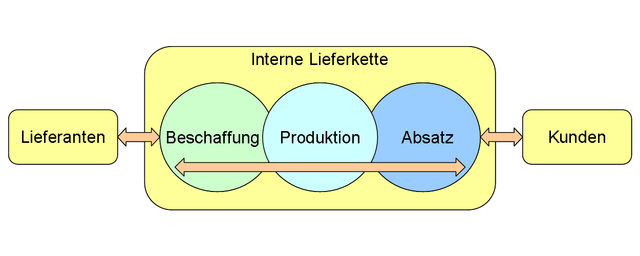
\includegraphics[width=0.6\textwidth]{../pics/Lieferkette}
\end{figure}

\section{Das SCM Haus}
Um die zahlreichen Facetten von Supply Chain Management aufzuzeigen, werden die einzelnen Elemente in einem Haus zusammen gefasst.

Um ein stabiles Haus bauen zu können, wird starkes Fundament benötigt. In unserem Fall bestehen die Grundmauern aus den verschiedensten Abteilungen, Aufgaben und Prozesse im gesamtem Unternehmen.

	
	% Beginn Module SAP APO
	\chapter{Die Module des SAP APO-Systems}
Die Planungslandschaft in SAP APO lässt sich in mehrere Funktionsmodulen unterteilen:
\begin{itemize}
	\item Demand Planing (DP)
	\item Supply Network Planning (SNP)
	\item Production Planning/Detailed Scheduling (PP/DS)
	\item Global Available-to-Promise (ATP)
	\item Transport Load Builder (TLB)
\end{itemize}

\section{Demand Planning (DP)}

\subsection{Konstantmodell}
Das vom Demand Plannung Tool zur Verfügung gestellte Konstantmodell ist die exponentielle Glättung 1. Ordnung. Für dieses Prognosemodell werde folgende Größen benötigt \cite[S.~138~ff]{Stadtler:2010:SCM:1965255}:
\begin{enumerate}
	\item den aktuellen Zeitreichenwert \(x_{(t)}\)
	\item der letzte Vergangenheitswert \(x_{(t-1)}\)
	\item sowie der Glättungsfaktor Alpha (\(\alpha\))
\end{enumerate}
Die Formel zu Berechnung einer Periode lautet:
\begin{equation}
	x_{(t+1)} = \alpha * x_{(t)} + (1 - \alpha) * x^*_{(t-1)} 
\end{equation}
Im Gegensatz zum gleitenden Mittel werden alle beobachteten Werte mit dem Glättungsfaktor versehen. Dieser steuert die Gewichtung der einzelnen Werte und gibt an ob der Schwerpunkt in den vergangenen Werten liegt oder in den neueren.
Um mehrere Vergangenheitswerte in die Formel einfließen zu lassen, wir der letzte Teil des mathematischen Ausdrucks um eine Rekursion erweitert:
\begin{equation}
(1 - \alpha) * x_{(t-1)} + \alpha(1 - \alpha)^{2} * x_{(t-2)} + ... + \alpha(1 - \alpha)^{t-1} * x_{1} + (1-a)^t * x_0
\end{equation}
Werden mehrere vergangene Werte in die Formel eingefügt, dann nimmt deren Gewichtung exponentiell ab. Wird als Beispiel der Alpha Faktor 0,5 gewählt, so werden die Vergangenheitswerte wie folgt bewertet:
\begin{itemize}
	\item 1. Vergangenheitswert 50 \%
	\item 2. Vergangenheitswert 25 \%
	\item 3. Vergangenheitswert 12,5 \%
	\item 4. Vergangenheitswert 6,25 \%
\end{itemize}
Der Alpha Faktor kann einen Wert in folgendem Bereich annehmen:
$ 0 \leq \alpha \leq 1 $
Mit diesem Wissen lässt sich für die Wahl des Alpha Faktors folgenden herleiten:
Wird $\alpha$ niedrig gewählt, dann verschiebt sich die Gewichtung auf vergangene Werte. Ein großer Alpha Wert jedoch gewichtet die Werte der heutigen und jüngsten Vergangenheit stärker. Das liegt daran, dass durch den exponentiellen Verfall der Formel diese schneller an Gewichtung verlieren. Ein kleiner Alpha Wert hat zur Folge, dass Zufallsschwankungen eher gedämpft werden und erhöht die Stabilität der Prognose.

\subsection{Lineare Regression}
Das Trendmodell setzt, wie im Namen schon angedeutet, einen Trend in den beobachteten Vergangenheitswerten voraus. Durch die vergangenen Werte wird eine Gerade gezogen. Diese Vorgehensweise zu Bestimmung der Trendgerade ist die der Kleinsten Quadrate (KQ).
Die Position der Gerade wird so bestimmt, das die Summe der Abweichungsquadrate, zwischen den beobachteten Werten und Gerade minimal sind. Die zu ermittelnde Funktion hat die Form \cite{schwarze2009}:
\begin{equation}
	f(x) = a + bx
\end{equation}
Die zwei Koeffizienten, a und b, lassen sich mit den folgenden zwei Funktionen ermitteln:
\begin{equation}
	a = \dfrac{\Sigma x^{2}_{i} \Sigma y_{i} - \Sigma x_{i} \Sigma x_{i}y_{i}}{n \Sigma x^{2}_{i} - (\Sigma x_{i})^{2}}
\end{equation}

\begin{equation}
	b = \dfrac{n\Sigma x_{i}y_{i} - \Sigma x_{i} \Sigma y_{i}}{n \Sigma x^{2}_{i} - (\Sigma x_{i})^{2}}
\end{equation}
Die Beschreibung der einzelnen mathematischen Zeichen lautet wie folgt:
\begin{itemize}
	\item \(x_{i}\) = Periode an der Stelle i
	\item \(y_{i}\) = Absatz in der Periode i
	\item n = Anzahl der betrachteten Perioden
	\item f(x) = Lineare KQ-Regressionsfunktion
\end{itemize}
Nachdem die Regressionsfunktion ermittelt wurde, kann die Prognose für einen beliebigen Zukunftswert durchgeführt werden. Dazu muss "f(x)" durch die gewünschte Periode ersetzt und die Funktion nach "x" aufgelöst werden.

\subsection{Saisonmodell}
Saisonale Absatzmodelle sind Gütern zuzuordnen, welche aufgrund der Jahreszeit in ihrem Absatz schwanken. Das können Kleidungsartikel (Wintermode), Speisen (Spargel) oder Reisen (Karibikurlaub) sein um einige Beispiele zu nennen.
Um saisonale Einflüsse erkennen zu können, müssen die Vergangenheitswerte auf folgende Merkmale hin untersucht werden \cite[S.~25]{Larouque2010}:
\begin{itemize}
	\item Regelmäßige Schwankungen zu bestimmten Zeiten des Jahres/Quartals/Monats
	\item Äußere Einflüsse sind maßgebend für den Bedarf (Weihnachten, Urlaub, etc.)
	\item Bedarfsspitzen und -täler müssen in einem vergleichbarem Zeitraum (Periode) stattfinden. Das gilt der Abgrenzung von zufälligen Schwankungen
	\item Eine Schwankung muss einem eindeutigem Anlasse vorliegen, der auch in Zukunft bestand hat.
	\item Die Abweichung muss bedeutend größer sein als die zufälligen Schwankungen
\end{itemize}
Aus den oben genannten Gründen ist es wichtig, dass ein saisonaler Bedarf erst bei Betrachtung mehrerer Saisonzeiträume (mindestens zwei) möglich ist.

\subsection{Trendsaisonmodell}
\subsection{Sporadisches/unregelmäßiges Modell}

\section{Supply Network Planning}
\cite[S.~169~ff]{Witt:2014:GrundkursSAPAPO}
\section{Production Planning and Detailed Scheduling}
\section{Global Available-to-Promise}
\section{Transport Load Builder}

	
	
	 % Beginne mit Anhang
	\newpage
	% Abbilungsverzeichnis ins Inhaltsverzeichnis aufnehmen
	\addcontentsline{toc}{chapter}{Abbildungsverzeichnis}
	\fancyhead[L]{Abbildungs- / Tabellen- / Listingverzeichnis}
	% Abbildungsverzeichnis anzeigen
	\listoffigures

	\newpage
	% Literaturliste soll im Inhaltsverzeichnis auftauchen
	\addcontentsline{toc}{chapter}{Literaturverzeichnis}
	% Literaturverzeichnis anzeigen
	\renewcommand\refname{Literaturverzeichnis}
	\fancyhead[L]{\nouppercase{\leftmark}} 
	\bibliography{../chapters/99_literature}
	% Stil und Art der Zitierung
	\bibliographystyle{alphadin} % deutsch, Sortierung nach Kürzel des Autors, Referenz nach Kürzel des Autors und Jahreszahl
	% Ende Anhang

\end{document}
